\RequirePackage[l2tabu, orthodox, abort]{nag}
\documentclass[a4paper, 11pt]{article}

\usepackage[utf8x]{inputenc}
\usepackage[T1]{fontenc}
\usepackage{ucs}
\usepackage[english]{babel}
\usepackage{mathtools, amsmath, amsfonts, amssymb}
\usepackage{fancyhdr}
\usepackage{graphicx}
\usepackage[sc]{mathpazo}
\usepackage[scaled]{beramono}
\usepackage[scaled]{helvet}
\usepackage{float}
\usepackage[font={small,it}]{caption}
\usepackage{fixltx2e}
\usepackage{bm}
\usepackage{fullpage}
\usepackage{verbatim}
\usepackage{subcaption}
\usepackage[noabbrev]{cleveref}
\usepackage{booktabs}
% \usepackage[parfill]{parskip}

% \usepackage[colorinlistoftodos]{todonotes}
% \usepackage{xfrac}
% \usepackage{array}
% \usepackage{booktabs}

\linespread{1.05}
\pagestyle{fancyplain}
\fancyhead{}
\fancyfoot[L]{}
\fancyfoot[C]{}
\fancyfoot[R]{\thepage}
\renewcommand{\headrulewidth}{0pt}
\renewcommand{\footrulewidth}{0pt}
\setlength{\headheight}{13.6pt}

\widowpenalty=9000
\clubpenalty=9000

\newcommand{\horrule}[1]{\rule{\linewidth}{#1}}
\newcommand{\vect}[1]{\mathbf{#1}}
\newcommand{\mat}[1]{\textbf{#1}}

% Todonotes commands.
\newcommand{\addref}{\todo[color=red!40]{Add reference.}}
\newcommand{\rewrite}[1]{\todo[color=green!40]{#1}} 
\newcommand{\missing}[1]{\todo[inline,color=green!40]{Need to write: #1}}

\title{ 
\normalfont\normalsize 
\textsc{University of Copenhagen} \\ [25pt]
\horrule{0.5pt} \\[0.4cm]
\huge StatML\@: Exam 2014\\
\horrule{2pt} \\[0.5cm]
}

\author{Jens Fredskov (chw752)}

\begin{document}
\maketitle
\pagebreak

\section{Predicting the Specific Star Formation Rate} % (fold)
\label{sec:predicting_the_specific_star_formation_rate}

\subsection*{Question 1}
For the this question a maximum likelihood linear regression has been used. This means the basis functions used were linear such that $\phi_j(\mathbf{x}) = x_j$, except for the first function which were $\phi_0(\mathbf{x}) = 1$, as this is a dummy function to allow a bias. When applying the maximum likelihood method\footnote{This is simply using $\mathbf{w}_{\mathit{ML}} = \bm\Phi^\dagger t$, where $\bm\Phi^\dagger$ is the Moore-Penrose pseudo-inverse of $\bm\Phi$ and $t$ is the target of our data.} using a classic design matrix $\bm\Phi$ constructed from the basis functions and the data from the training set, I got a weight vector
\[
    \mathbf{w}_{\mathit{ML}} = \begin{pmatrix}
      -8.1494 \\
       -0.794 \\
       -1.223 \\
     -0.32858 \\
     -0.78633 \\
    \end{pmatrix}
    \label{eq:wml}
\]
which when applied to the data gave mean squared errors of
\begin{align*}
    \mathrm{MSE}_{\mathit{train}} &= 0.27475 \\
    \mathrm{MSE}_{\mathit{test}} &= 0.27518
\end{align*}

The error of the two sets is almost equal, which suggests that we probably have not over-fitted to the training data. Furthermore the error is reasonably small, leading to the conclusion that a linear model, might be a good choice of model for our data.
% TODO Possibly extend with a paragraph about not having done sufficient validation to ensure linear is a good model

The source code used in the implementation of this question can be found in \texttt{question1.m}, \texttt{linearRegression.m} and \texttt{meanSquaredError.m}.

\subsection*{Question 2} % FIXME This question has NOT been answered yet
\begin{comment} % REMOVE THIS WHEN READY
\begin{figure}[H]
    \centering
    \includegraphics[width=0.8\textwidth]{figures/question2}
    \caption{Here be dragons.}\label{fig:question2}
\end{figure}

degree of polynimium = 3
\begin{align*}
    \mathrm{MSE}_{\mathit{train}} &= 0.25635 \\
    \mathrm{MSE}_{\mathit{test}} &= 0.25835
\end{align*}

Notes: we could also do regularisation, and/or radial/polynomial basis functions.

The source code used in the implementation of this question can be found in \texttt{question2.m}, \texttt{polyRegression.m}, \texttt{polyPredict.m}, \texttt{meanSquaredError.m} and \texttt{betterPlots.m}.
\end{comment} % REMOVE THIS WHEN READY

% section predicting_the_specific_star_formation_rate (end)

\section{Stars vs. Galaxies} % (fold)
\label{sec:stars_vs_galaxies}

\subsection*{Question 3}
I have made use of the \texttt{libsvm-3.17}\footnote{http://www.csie.ntu.edu.tw/\textasciitilde{}cjlin/libsvm/} to perform the standard C-SVM binary classification.

Using the described Jaakkola's heuristic I calculated the initial value for $\sigma$ and afterwards for $\gamma$, using the identity
\[
    \sigma = \sqrt{1 / (2 \gamma)} \Leftrightarrow \gamma = 1 / (2 \sigma^2)
\]

The initial values suggested by the heuristic was
\[
    \sigma_{\mathit{jaakkola}} = 1.8119,\quad \gamma_{\mathit{jaakkola}} = 0.1523
\]

Using these I performed a grid search to determine the appropriate hyper parameters for the SVM\@. The grid search was set up such that all the given combinations was tried, for each of the three given bases. That I tried every combination of the type
\[
    \lbrace C \times \gamma \rbrace \in \lbrace b^i \times \gamma_{\mathit{jaakkola}} \cdot b^j | -2 \le i \le 3 \wedge -3 \le j \le 3 \wedge b \in \lbrace 2, e, 10 \rbrace \rbrace
\]
On every combination 5-fold cross validation was performed, and the one with the lowest average 0--1 loss was then chosen to be the best hyper parameters. The cross validation splits the data into the five folds by sorting the data on class and then evenly distributing the using modulo (such that every fold gets one of the first five data points, one of the five next, and so on). This is done to ensure that every fold is representative of the entire data set.

Using this method the hyper parameters was found to be
\[
    C = 1000 \quad \gamma = 0.001523
\]
with a base of $10$, so $C = 10^3$ and $\gamma = \gamma_{\mathit{jaakkola}} \cdot 10^{-2}$.

These hyper parameters and the training data were then used to train the SVM\@. The classification error on the training and test data when using the trained SVM was then
\begin{align*}
    \mathrm{Accuracy}_{\mathit{train}} &= 0.997333 = 99.73 \% \\
    \mathrm{Accuracy}_{\mathit{test}} &= 0.996333 = 99.63 \%
\end{align*}

The source code used in the implementation of this question can be found in \texttt{question3.m}, \texttt{jaakkola.m}, \texttt{crossValidation.m} and \texttt{svmClassify.m}.

\subsection*{Question 4}
To perform the PCA I have not used any libraries (e.g.\ the built in MATLAB function \texttt{pca}). The analysis was performed by first computing the covariance matrix of the data, and then the eigenvectors and -values by using. Both of these computations can be done with built in functions \texttt{cov} and \texttt{eig} of MATLAB\@. Afterwards I simply sorted the eigenvectors, by their eigenvalue. The corresponding eigenspectrum can be seen in \Cref{fig:question4_1}. As can be seen almost all of the variance is caught by the first two principal components. 

\begin{figure}[H] % TODO add proper captions
    \centering
    \begin{subfigure}[b]{0.49\textwidth}
    \includegraphics[width=\textwidth]{figures/question4_1}
        \caption{Here be dragons.}\label{fig:question4_1}
    \end{subfigure}
    \begin{subfigure}[b]{0.49\textwidth}
        \includegraphics[width=\textwidth]{figures/question4_2}
        \caption{Here be dragons.}\label{fig:question4_2}
    \end{subfigure}
    \caption{Here be dragons}\label{fig:question4}
\end{figure}

In \Cref{fig:question4_2} the data points have been plotted after being projected on the first two principal components. As can be seen we do get a split of the two classes. However many star-class data points lie inside the galaxy-class. So while the the projection does provide at decent split, it is by no means perfect, and without the colouring of classes on might have thought the classes were divided by a horizontal line at around 62.5, as there is what seems to be a hole between two groups of points there.

The source code used in the implementation of this question can be found in \texttt{question4.m}, \texttt{pca.m} and \texttt{betterPlots.m}.

\subsection*{Question 5}
To perform the 2-means clustering I have used the built in MATLAB function \texttt{kmeans}. This function applies the iterative k-means algorithm and seeks to minimise the sum, over all clusters, of the within-cluster sums of point-to-cluster-centroid distances. The functions was set to perform 100 attempts with different starting points for the clusters. These starting points are by the function chosen as random sample points, which in general serve as better guesses than completely random points in the entire $\mathbb{R}^2$. To ensure consistent results the seed for randomisation is set beforehand (any number could be chosen, but here I have used $43786953$ which has no special meaning). The 10-dimensional centres found using this method can be found in \Cref{tab:question4}.

\begin{table}[H]
    \centering
    \begin{tabular}{lcc}
        \toprule
        Feature name & $c_1$ & $c_2$ \\
        \midrule
        cModelMag\_u & 19.324 & 22.349 \\
        cModelMag\_g & 17.971 & 21.413 \\
        cModelMag\_r & 17.291 & 20.290 \\
        cModelMag\_i & 16.965 & 19.599 \\
        cModelMag\_z & 16.774 & 19.222 \\
        psfModelMag\_u & 20.297 & 23.451 \\
        psfModelMag\_g & 18.876 & 22.096 \\
        psfModelMag\_r & 18.201 & 20.946 \\
        psfModelMag\_i & 17.880 & 20.272 \\
        psfModelMag\_z & 17.647 & 19.855 \bottomrule
    \end{tabular}
    \caption{Here be dragons.}\label{tab:question4}
\end{table}

When projecting these on the first two principal components of the data its look as in \Cref{fig:question5}, where \Cref{fig:question5_1} shows the classes as guessed by the 2-means clustering and \Cref{fig:question5_2} shows the actual classes.

\begin{figure}[H] % TODO add proper captions
    \centering
    \begin{subfigure}[b]{0.49\textwidth}
    \includegraphics[width=\textwidth]{figures/question5_1}
        \caption{Here be dragons.}\label{fig:question5_1}
    \end{subfigure}
    \begin{subfigure}[b]{0.49\textwidth}
        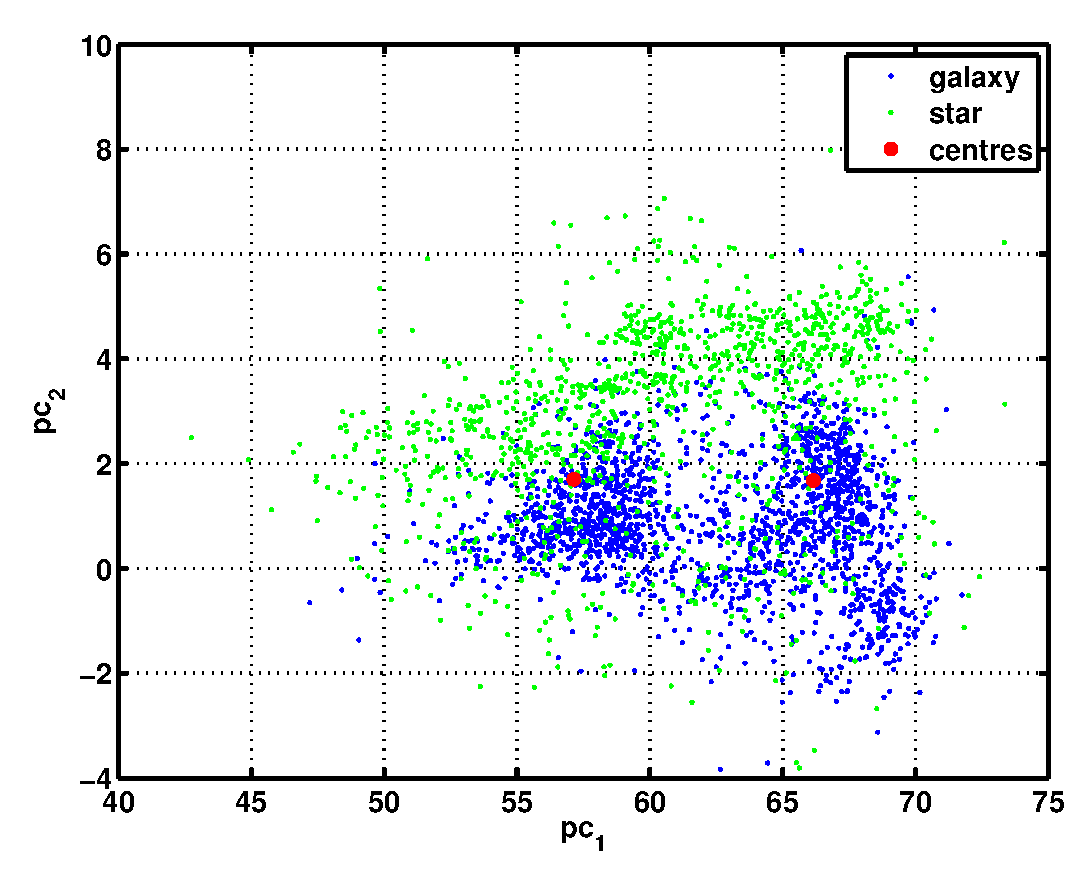
\includegraphics[width=\textwidth]{figures/question5_2}
        \caption{Here be dragons.}\label{fig:question5_2}
    \end{subfigure}
    \caption{Here be dragons.}\label{fig:question5}
\end{figure}

As can be seen the 2-means clustering did not find the correct split of the two classes. The split found however makes sense, as the galaxy-class seems to be split in two clusters, with the star-class lying above. Thus it makes sense that the split was performed as seen in \Cref{fig:question5}. In general the problem with the two classes is that one is very spread out on the first axis and lies just up to the second class which lies in two compact clusters. There clusters could therefore still be seen as meaningful, as they do represent some sort of split which seem to be present in the data, but they do not represent the split between the star- and galaxy-class very well.

% TODO Possibly add something about that we only see two pcs of the clusters so that the might actually be better, but that we have also looked at 3d which clearly shows that the clusters found are the two galxy-class clusters.

The source code used in the implementation of this question can be found in \texttt{question5.m} and \texttt{betterPlots.m}. Note that \texttt{question5.m} depends on \texttt{question4.m} and thus it is necessary to run this script beforehand. If the the questions are not run one at a time, but using the main script \texttt{main.m} this is already taken care of.

\subsection*{Question 6} %FIXME This has not been done yet!

% section stars_vs_galaxies (end)

\section{Variable Stars} % (fold)
\label{sec:variable_stars}

\subsection*{Question 7} % FIXME This has not been done yet!

Linear classification
\begin{align*}
    E_{\mathit{train}} &= 0.18418 \\
    E_{\mathit{test}} &= 0.28664
\end{align*}

Nonlinear classification
\[
    k_{\mathit{best}} = 6
\]
\begin{align*}
    E_{\mathit{train}} &= 0.44877 \\
    E_{\mathit{test}} &= 0.55512
\end{align*}

Notes: used LDA and KNN\@. KNN used 5-fold cross-val to choose K

The source code used in the implementation of this question can be found in \texttt{question7.m}, \texttt{trainLDA.m}, \texttt{kNN.m} and \texttt{crossValidation.m}.

\subsection*{Question 8} %FIXME This has not been done yet!

% section variable_stars (end)
\end{document}